\section{Proceso} 

\begin{itemize}
	\item Relacion entre tablas del excel
	\begin{center}
	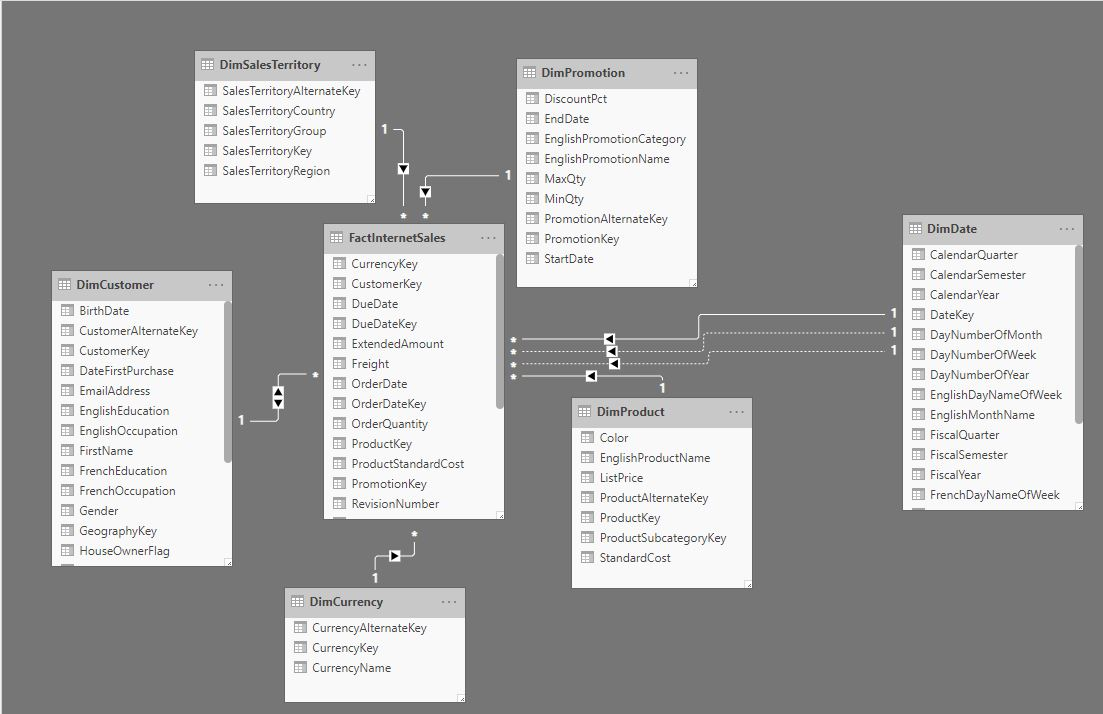
\includegraphics[width=10cm]{./Imagenes/1} 
	\end{center}
\end{itemize} 

\begin{itemize}
	\item Relacion de las tablas despues de agregar el nuevo excel
	\begin{center}
	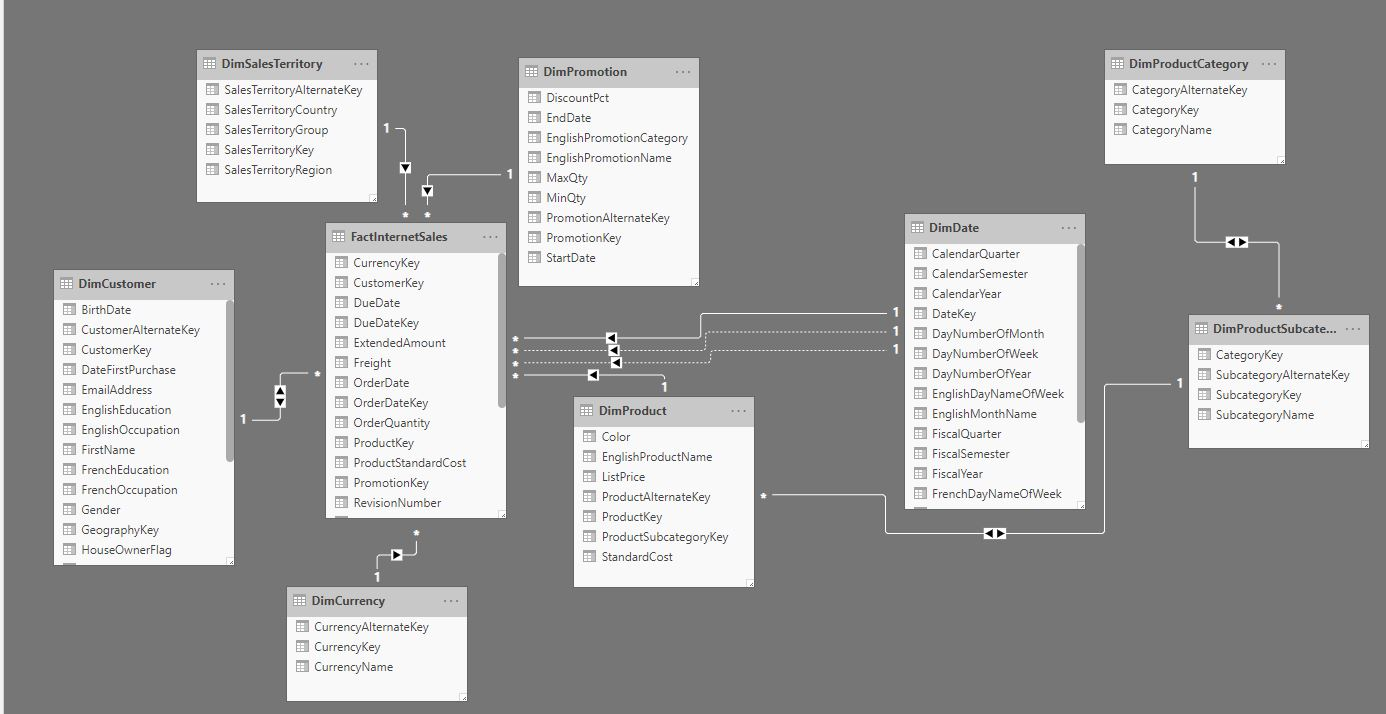
\includegraphics[width=10cm]{./Imagenes/2} 
	\end{center}
\end{itemize} 

\begin{itemize}
	\item Calculo de columna en DimCustomer
	\begin{center}
	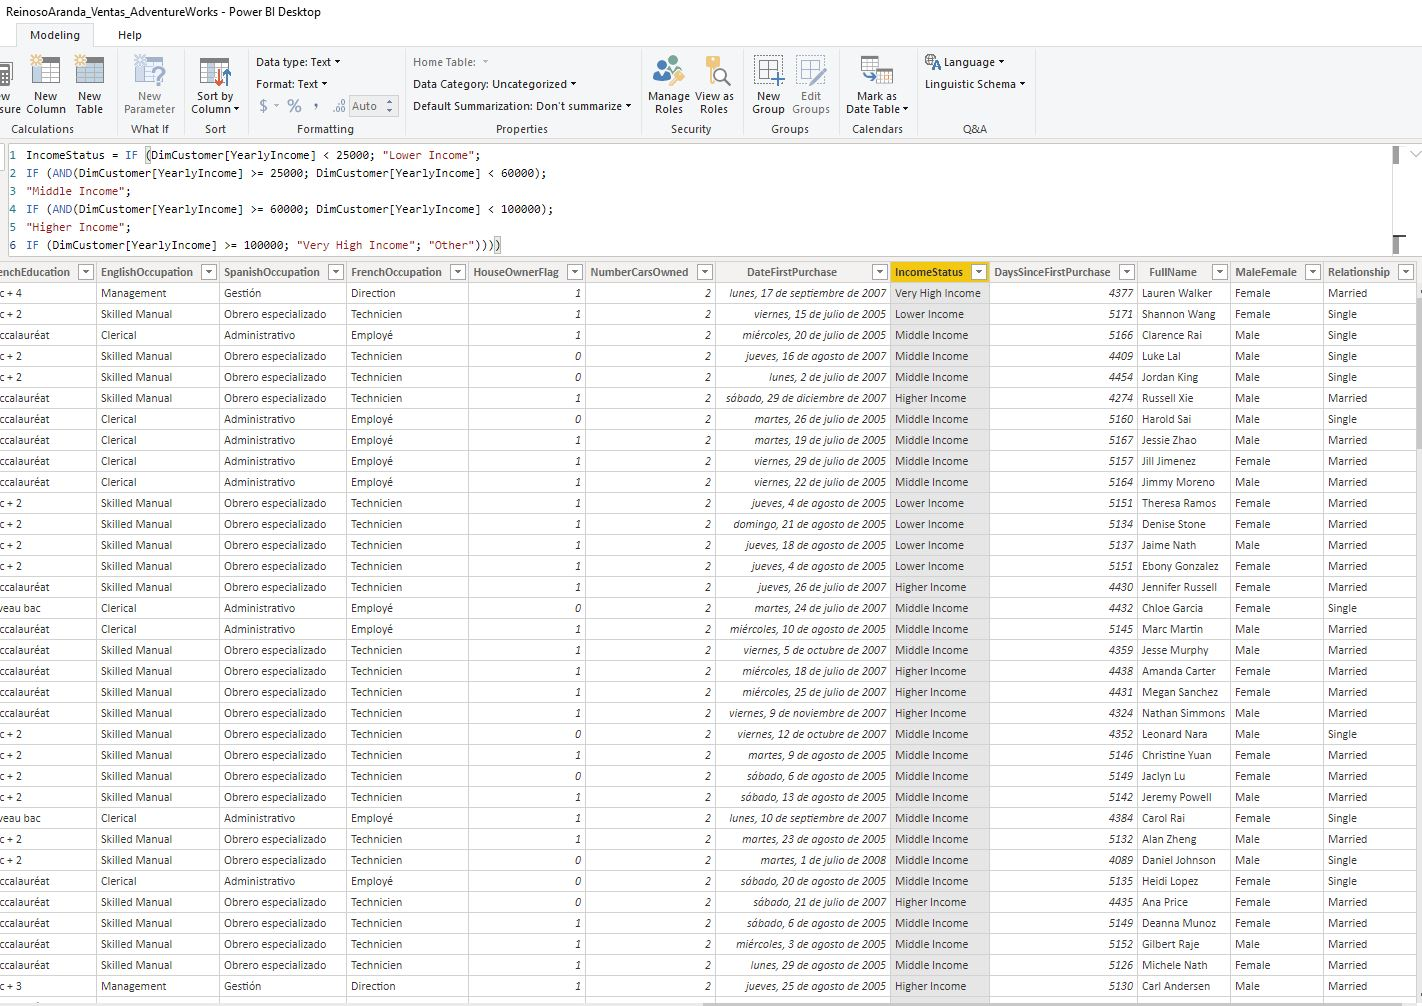
\includegraphics[width=10cm]{./Imagenes/3} 
	\end{center}
\end{itemize} 

\begin{itemize}
	\item Relaciones de las tablas
	\begin{center}
	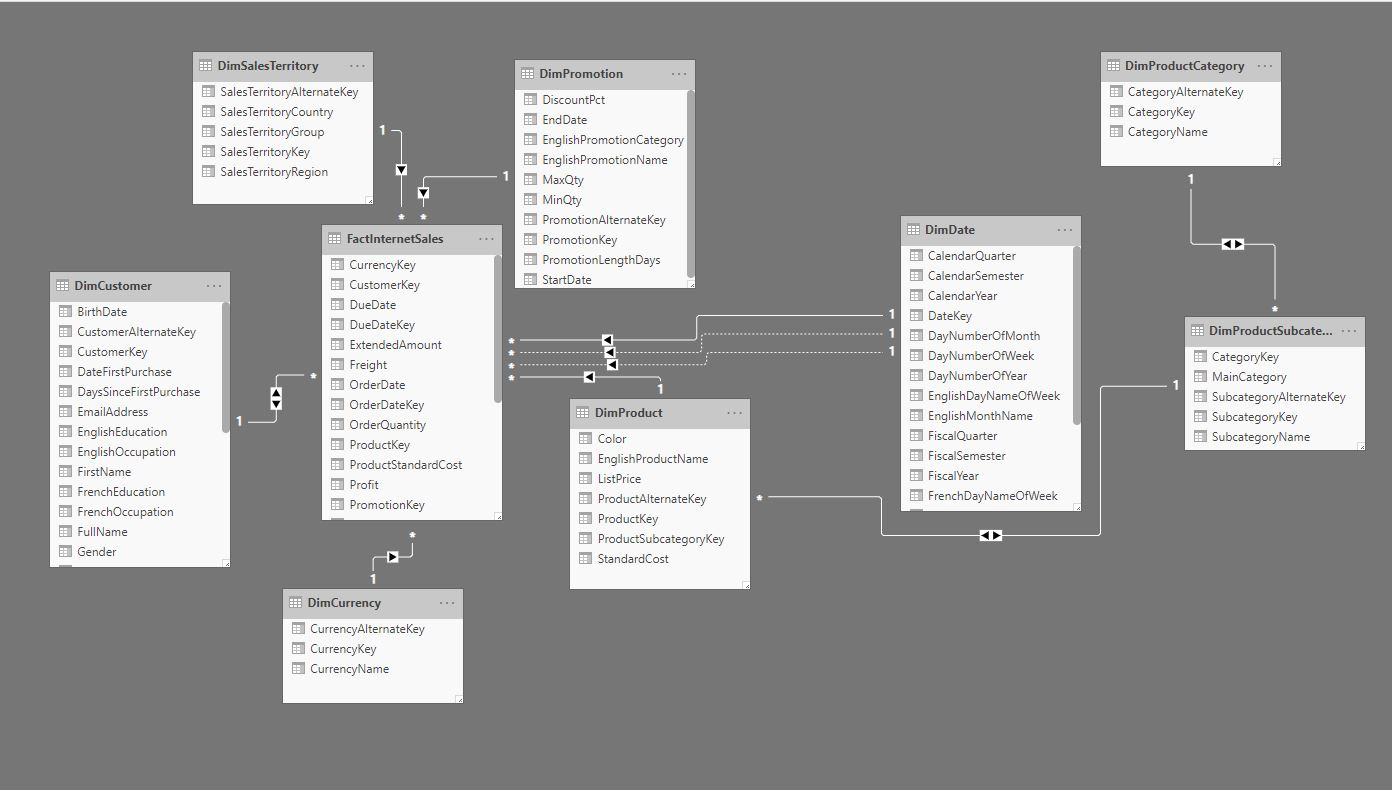
\includegraphics[width=10cm]{./Imagenes/4} 
	\end{center}
\end{itemize} 

\begin{itemize}
	\item Calculo en una columna en la tabla DimProductSubcategory
	\begin{center}
	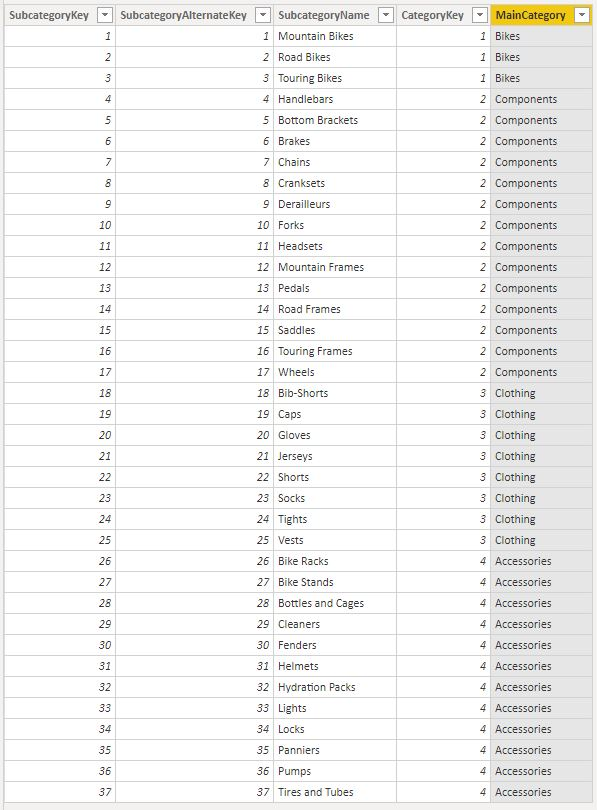
\includegraphics[width=10cm]{./Imagenes/5} 
	\end{center}
\end{itemize} 

\begin{itemize}
	\item Calculo en una columna en la tabla DimPromotion
	\begin{center}
	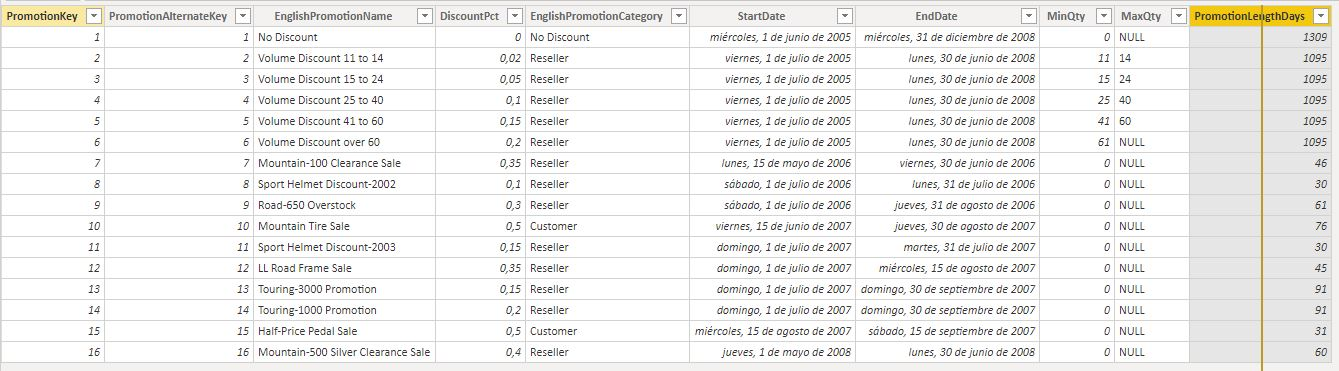
\includegraphics[width=10cm]{./Imagenes/6} 
	\end{center}
\end{itemize} 

\begin{itemize}
	\item Calculo en una columna en la tabla FactInternetSales
	\begin{center}
	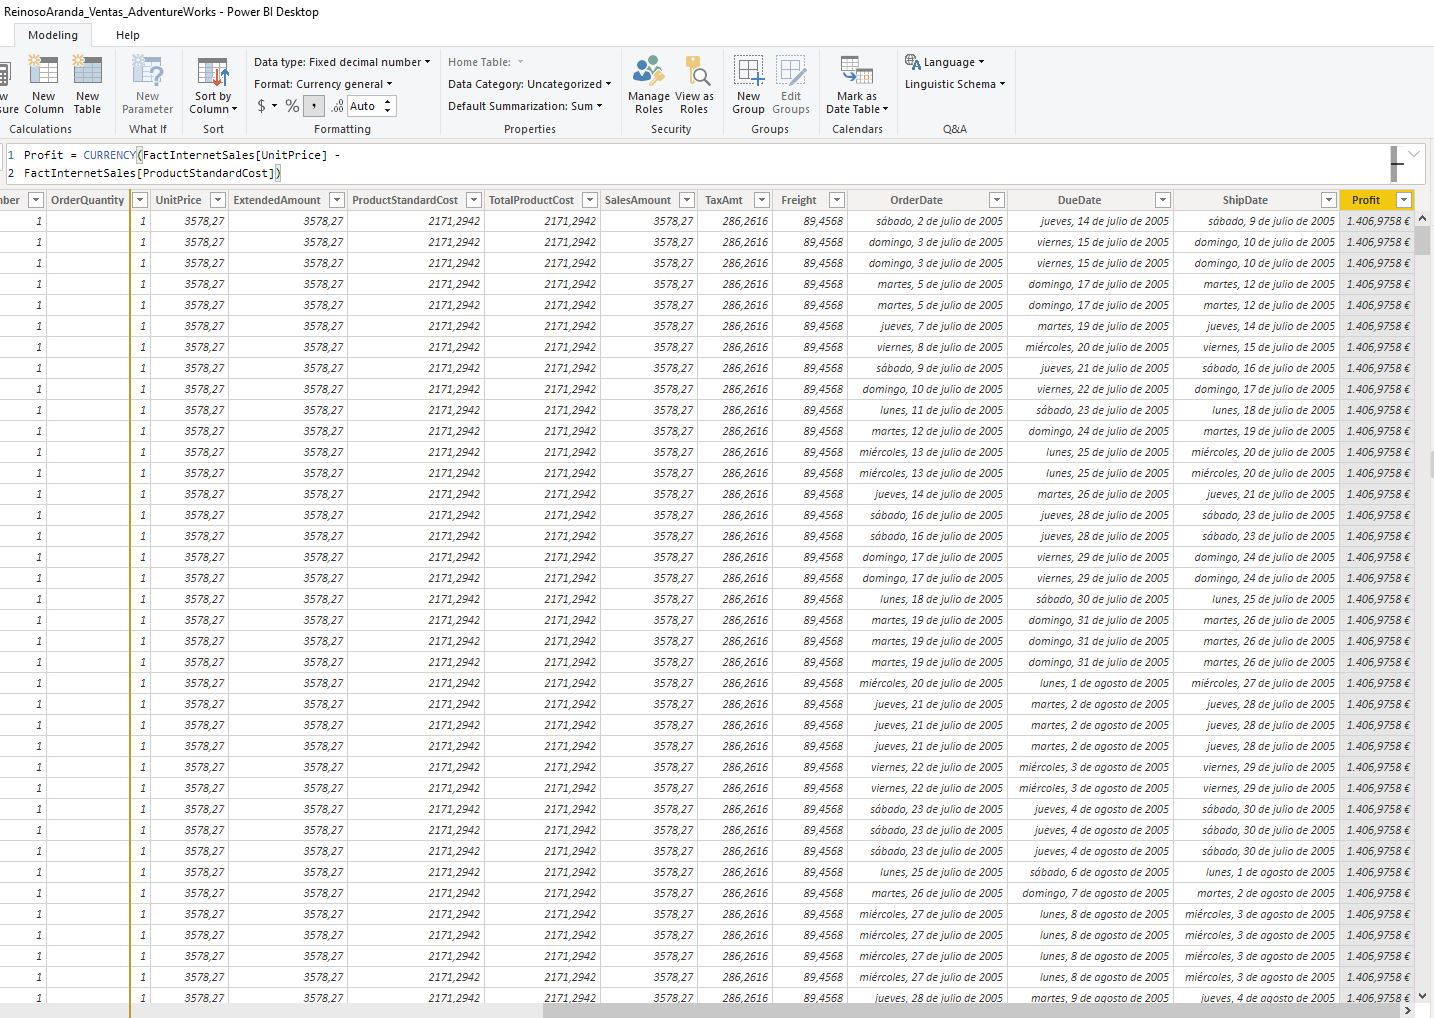
\includegraphics[width=10cm]{./Imagenes/7} 
	\end{center}
\end{itemize} 